\begin{figure*}[t]
  \centering

  \tikzstyle{plain} = [circle, fill=white, text=black, draw, thick, scale=1, minimum size=0.5cm, inner sep=1.5pt]
  \tikzstyle{small} = [circle, fill=white, text=black, draw, thick, scale=1, minimum size=0.2cm, inner sep=1.5pt]
  \tikzstyle{thickedge} = [line width=0.8mm]

  \begin{minipage}[m]{.32\textwidth}
      \vspace{0pt}
      \centering
      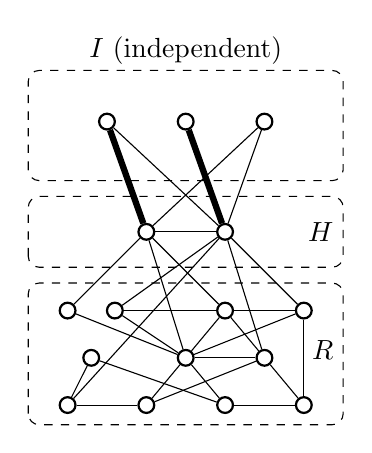
\begin{tikzpicture}
          % vertices
          \node[small] (r1) at (1, 1.8) {};
          \node[small] (r2) at (2, 1.8) {};
          \node[small] (r3) at (3, 1.8) {};
          \node[small] (r4) at (4, 1.8) {};

          \node[small] (r5) at (1.3, 2.4) {};
          \node[small] (r6) at (2.5, 2.4) {};
          \node[small] (r7) at (3.5, 2.4) {};

          \node[small] (r8) at (1, 3) {};
          \node[small] (r9) at (1.6, 3) {};
          \node[small] (r10) at (3, 3) {};
          \node[small] (r11) at (4, 3) {};

          \node[small] (c1) at (2, 4) {};
          \node[small] (c2) at (3, 4) {};

          \node[small] (b1) at (1.5, 5.4) {};
          \node[small] (b2) at (2.5, 5.4) {};
          \node[small] (b3) at (3.5, 5.4) {};

          % edges
          \draw (r1) -- (r2);
          \draw (r3) -- (r4);
          \draw (r1) -- (r5);
          \draw (r2) -- (r6);
          \draw (r2) -- (r7);
          \draw (r3) -- (r5);
          \draw (r3) -- (r6);
          \draw (r4) -- (r7);
          \draw (r6) -- (r7);
          \draw (r6) -- (r8);
          \draw (r6) -- (r9);
          \draw (r6) -- (r10);
          \draw (r6) -- (r11);
          \draw (r7) -- (r10);
          \draw (r4) -- (r11);
          \draw (r9) -- (r10);
          \draw (r10) -- (r11);

          \draw (r8) -- (c1);
          \draw (r6) -- (c1);
          \draw (r10) -- (c1);
          \draw (r7) -- (c2);
          \draw (r9) -- (c2);
          \draw (r11) -- (c2);
          \draw (r1) -- (c2);

          \draw (c1) -- (c2);
          \draw[thickedge] (c1) -- (b1);
          \draw (c1) -- (b3);
          \draw (c2) -- (b1);
          \draw[thickedge] (c2) -- (b2);
          \draw (c2) -- (b3);

          % annotation
          \draw[rounded corners, dashed] (0.5, 1.55) rectangle ++ (4, 1.8);
          \node[anchor=east] at (4.5, 2.5) {$R$};

          \draw[rounded corners, dashed] (0.5, 3.55) rectangle ++ (4, 0.9);
          \node[anchor=east] at (4.5, 4) {$H$};

          \draw[rounded corners, dashed] (0.5, 4.65) rectangle ++ (4, 1.4);
          \node[] at (2.5, 6.3) {$I$ (independent)};
      \end{tikzpicture}
  \end{minipage}
  \hfill
%
  \begin{minipage}[m]{.32\textwidth}
    \vspace{0pt}
    \centering
    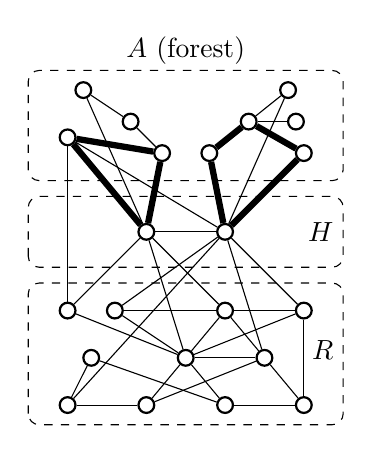
\begin{tikzpicture}
        % vertices
        \node[small] (r1) at (1, 1.8) {};
        \node[small] (r2) at (2, 1.8) {};
        \node[small] (r3) at (3, 1.8) {};
        \node[small] (r4) at (4, 1.8) {};

        \node[small] (r5) at (1.3, 2.4) {};
        \node[small] (r6) at (2.5, 2.4) {};
        \node[small] (r7) at (3.5, 2.4) {};

        \node[small] (r8) at (1, 3) {};
        \node[small] (r9) at (1.6, 3) {};
        \node[small] (r10) at (3, 3) {};
        \node[small] (r11) at (4, 3) {};

        \node[small] (c1) at (2, 4) {};
        \node[small] (c2) at (3, 4) {};

        \node[small] (b1) at (2.2, 5) {};
        \node[small] (b2) at (1.8, 5.4) {};
        \node[small] (b3) at (1.2, 5.8) {};
        \node[small] (b4) at (1, 5.2) {};

        \node[small] (b5) at (2.8, 5) {};
        \node[small] (b6) at (3.3, 5.4) {};
        \node[small] (b7) at (4, 5.0) {};
        \node[small] (b8) at (3.9, 5.4) {};
        \node[small] (b9) at (3.8, 5.8) {};

        % edges
        \draw (r1) -- (r2);
        \draw (r3) -- (r4);
        \draw (r1) -- (r5);
        \draw (r2) -- (r6);
        \draw (r2) -- (r7);
        \draw (r3) -- (r5);
        \draw (r3) -- (r6);
        \draw (r4) -- (r7);
        \draw (r6) -- (r7);
        \draw (r6) -- (r8);
        \draw (r6) -- (r9);
        \draw (r6) -- (r10);
        \draw (r6) -- (r11);
        \draw (r7) -- (r10);
        \draw (r4) -- (r11);
        \draw (r9) -- (r10);
        \draw (r10) -- (r11);

        \draw (r8) -- (c1);
        \draw (r6) -- (c1);
        \draw (r10) -- (c1);
        \draw (r7) -- (c2);
        \draw (r9) -- (c2);
        \draw (r11) -- (c2);
        \draw (r1) -- (c2);

        \draw (c1) -- (c2);
        \draw[thickedge] (c1) -- (b1);
        \draw (c1) -- (b3);
        \draw[thickedge] (c1) -- (b4);
        \draw (c2) -- (b4);
        \draw[thickedge] (c2) -- (b5);
        \draw[thickedge] (c2) -- (b7);
        \draw (c2) -- (b9);

        \draw (b1) -- (b2);
        \draw (b2) -- (b3);
        \draw[thickedge] (b1) -- (b4);
        \draw[thickedge] (b5) -- (b6);
        \draw[thickedge] (b6) -- (b7);
        \draw (b6) -- (b8);
        \draw (b6) -- (b9);

        \draw (b4) -- (r8);

        % annotation
        \draw[rounded corners, dashed] (0.5, 1.55) rectangle ++ (4, 1.8);
        \node[anchor=east] at (4.5, 2.5) {$R$};

        \draw[rounded corners, dashed] (0.5, 3.55) rectangle ++ (4, 0.9);
        \node[anchor=east] at (4.5, 4) {$H$};

        \draw[rounded corners, dashed] (0.5, 4.65) rectangle ++ (4, 1.4);
        \node[] at (2.5, 6.3) {$A$ (forest)};
      \end{tikzpicture}
  \end{minipage}
  \hfill
%
  \begin{minipage}[m]{.32\textwidth}
    \vspace{0pt}
    \centering
    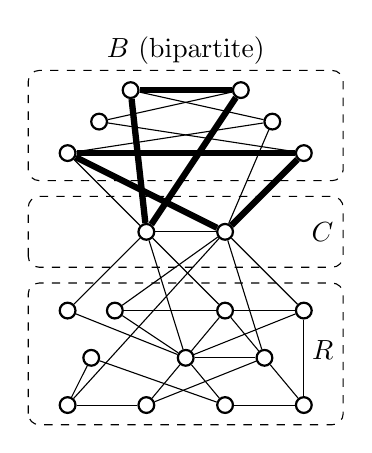
\begin{tikzpicture}
        % vertices
        \node[small] (r1) at (1, 1.8) {};
        \node[small] (r2) at (2, 1.8) {};
        \node[small] (r3) at (3, 1.8) {};
        \node[small] (r4) at (4, 1.8) {};

        \node[small] (r5) at (1.3, 2.4) {};
        \node[small] (r6) at (2.5, 2.4) {};
        \node[small] (r7) at (3.5, 2.4) {};

        \node[small] (r8) at (1, 3) {};
        \node[small] (r9) at (1.6, 3) {};
        \node[small] (r10) at (3, 3) {};
        \node[small] (r11) at (4, 3) {};

        \node[small] (c1) at (2, 4) {};
        \node[small] (c2) at (3, 4) {};

        \node[small] (b1) at (1, 5) {};
        \node[small] (b2) at (1.4, 5.4) {};
        \node[small] (b3) at (1.8, 5.8) {};

        \node[small] (b4) at (4, 5) {};
        \node[small] (b5) at (3.6, 5.4) {};
        \node[small] (b6) at (3.2, 5.8) {};

        % edges
        \draw (r1) -- (r2);
        \draw (r3) -- (r4);
        \draw (r1) -- (r5);
        \draw (r2) -- (r6);
        \draw (r2) -- (r7);
        \draw (r3) -- (r5);
        \draw (r3) -- (r6);
        \draw (r4) -- (r7);
        \draw (r6) -- (r7);
        \draw (r6) -- (r8);
        \draw (r6) -- (r9);
        \draw (r6) -- (r10);
        \draw (r6) -- (r11);
        \draw (r7) -- (r10);
        \draw (r4) -- (r11);
        \draw (r9) -- (r10);
        \draw (r10) -- (r11);

        \draw (r8) -- (c1);
        \draw (r6) -- (c1);
        \draw (r10) -- (c1);
        \draw (r7) -- (c2);
        \draw (r9) -- (c2);
        \draw (r11) -- (c2);
        \draw (r1) -- (c2);

        \draw (c1) -- (c2);
        \draw (c1) -- (b1);
        \draw[thickedge] (c1) -- (b3);
        \draw[thickedge] (c1) -- (b6);
        \draw[thickedge] (c2) -- (b1);
        \draw[thickedge] (c2) -- (b4);
        \draw (c2) -- (b5);

        \draw[thickedge] (b1) -- (b4);
        \draw (b1) -- (b5);
        \draw (b2) -- (b4);
        \draw (b2) -- (b6);
        \draw (b3) -- (b5);
        \draw[thickedge] (b3) -- (b6);

        % annotation
        \draw[rounded corners, dashed] (0.5, 1.55) rectangle ++ (4, 1.8);
        \node[anchor=east] at (4.5, 2.5) {$R$};

        \draw[rounded corners, dashed] (0.5, 3.55) rectangle ++ (4, 0.9);
        \node[anchor=east] at (4.5, 4) {$C$};

        \draw[rounded corners, dashed] (0.5, 4.65) rectangle ++ (4, 1.4);
        \node[] at (2.5, 6.3) {$B$ (bipartite)};
      \end{tikzpicture}
  \end{minipage}
%
  \caption{%
  Examples of crown decomposition (left),
  antler decomposition for \PrbFVSLong (middle) and 
  a tight OCC for \PrbOCTLong (right).
  Packings of forbidden subgraphs are highlighted in bold.
  }
  \label{fig:example}
\end{figure*}
